\section{Method}
\label{sec:method}

\subsection{Problem statement}

Let $\pi$ be a policy, $t$ a task of the suite and $s$ one of its stored initial states. The evaluator turns every rendered camera frame into a policy input through a pipeline $P$ of image steps. The outcome of the episode started from $(t, s)$ is $Y(\pi, P, t, s) \in \{0, 1\}$, and the success rate $S(\pi, P)$ is its mean over the $n$ evaluated pairs $(t, s)$. For a step $k$, the variant $P_{-k}$ differs from $P$ in step $k$ only, and the effect of the step is
\begin{equation}
\Delta_k(\pi) = S(\pi, P_{-k}) - S(\pi, P).
\end{equation}
Both pipelines start from the same initial states, so the estimate is paired. Let $L$ count the pairs that succeed under $P$ and fail under $P_{-k}$ (lost) and $G$ the reverse (gained), and let $f = L + G$ be the number of flips. Pairs with the same outcome cancel, and
\begin{equation}
\hat{\Delta}_k = \frac{G - L}{n}.
\end{equation}

\begin{figure}[t]
\centering
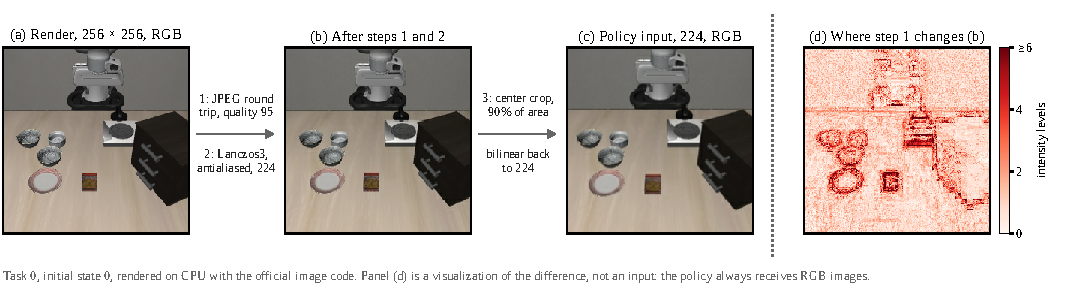
\includegraphics[width=\textwidth]{figures/pipeline.pdf}
\caption{The image steps of the official OpenVLA evaluation on LIBERO. (a) The RGB frame rendered by MuJoCo, after the \RotationDeg-degree rotation. (b) After step one, a JPEG encode and decode at quality \JpegQuality, and step two, a Lanczos3 resize to \InputRes{} with antialiasing. (c) The policy input after step three, a center crop of \CropAreaPct\% of the area resized back to \InputRes; the policy receives this RGB image. (d) A heat map of where step one changes image (b): for every pixel, the absolute change averaged over the R, G and B channels, in intensity levels. It visualizes the difference and is not an image any policy sees. The change sits on object edges, in $\DctBlock \times \DctBlock$ blocks, and its mean over the image is \FrameMeanDiff{} levels.}
\label{fig:pipeline}
\end{figure}

\subsection{The evaluation image pipeline}
\label{sec:pipeline}

We take the pipeline of the official OpenVLA evaluation on LIBERO as the reference (Figure~\ref{fig:pipeline}), as implemented in its code~\citep{openvlacode}. MuJoCo~\citep{mujoco} renders the third-person camera of the robosuite~\citep{robosuite} scene as a $\RenderRes \times \RenderRes$ RGB image, which is rotated by \RotationDeg{} degrees to match the training data. Step one encodes the image as JPEG with TensorFlow's default quality of \JpegQuality{} and decodes it immediately; a comment in the code states that this repeats the encoding of the dataset builder. Step two resizes the image to $\InputRes \times \InputRes$ with a Lanczos3 kernel~\citep{duchon1979} and antialiasing; the code comment states that this follows the resizing scheme of the Octo data loader~\citep{octo}, which OpenVLA uses for training. Step three keeps the central \CropAreaPct\% of the image area (each side scaled by \SideCrop) and resizes it back to \InputRes{} with bilinear interpolation; the evaluation code labels this crop as the counterpart of random-crop augmentation during training and asserts it for checkpoints trained with image augmentation. The environment is also seeded with a fixed value. OpenVLA-OFT~\citep{oft} applies the same steps to its third-person and wrist cameras~\citep{oftcode}. Every step keeps the three color channels.

Two properties explain why these steps may matter. JPEG~\citep{wallace1992} transforms each $\DctBlock \times \DctBlock$ block with the discrete cosine transform and quantizes the coefficients, high frequencies most coarsely, so its error concentrates in blocks that contain edges, which is where the outlines of the objects lie (Figure~\ref{fig:pipeline}d). Resizing changes the sampling grid: a kernel that is not low-pass enough lets high frequencies alias into the smaller image, and convolutional networks respond to such sampling details~\citep{azulay2019,zhang2019}. Lanczos and bilinear kernels filter differently, so the kernel can change the image a model sees.

\subsection{Variants}
\label{sec:variants}

Each variant changes one step and applies to every image the policy receives:
\begin{enumerate}
\item \emph{JPEG off}: the same TensorFlow resize call without the JPEG round trip;
\item \emph{Crop step off}: the evaluation script's own switch that skips step three. The policy then sees the full frame: objects appear about \Zoom\% smaller than in the center crop that matches training, and a band of about \Border{} pixels returns on each side;
\item \emph{Bilinear resize}: step two with the bilinear kernel, JPEG round trip and antialiasing unchanged;
\item \emph{Render at \InputRes}: the scene is rendered at $\InputRes \times \InputRes$, so step two no longer downsamples. The JPEG round trip and the Lanczos filter, now at scale one, are kept, so only the resolution changes. For OpenVLA-OFT this matches the official script, whose observation function applies the JPEG round trip and the resize to every frame before the model's own image preparation, which skips a second resize when an image is already at \InputRes~\citep{oftcode}; the harness logs the JPEG change of the first input in this cell (\OftRendMadMin{} to \OftRendMadMax{} intensity levels), which confirms that the round trip was applied.
\end{enumerate}
A fifth cell, the \emph{rerun}, repeats the reference unchanged. Before the variant cells ran, a check confirmed that the rewritten resize reproduces the official step pixel for pixel, so a variant differs from the reference in its one step only.

\subsection{Design choices}
\label{sec:design}

\emph{One step at a time.} Changing several steps together, as in earlier reproduction work~\citep{vlaevalrepo}, shows that the pipeline matters but not which step. Changing one step and keeping the rest attributes an effect to a step.

\emph{Paired episodes and a rerun.} LIBERO stores \NStates{} initial states per task, so a variant can be run from the same \NPairs{} states as the reference. Pairing removes the difference in difficulty between initial states from the comparison: only flips carry information, and the paired interval is narrower than an unpaired one (Appendix~\ref{app:ablation}). The rerun, an A/A comparison of the reference pipeline with itself, measures how many episodes change outcome when nothing changes on our stack.

\emph{Two policies with different action heads.} OpenVLA-7B picks each action dimension among \Bins{} discrete bins and acts one step per query; OpenVLA-OFT regresses continuous actions and executes chunks of \Chunk{} actions per query. Both start from the same vision backbone, so a difference in sensitivity between them may point to the action head and the decoding; the models also differ in their inputs (OpenVLA-OFT adds a wrist camera and the robot state) and in their fine-tuning, so this is a lead, not an attribution.

\emph{Color inputs.} The policies always receive RGB images, and we measure the size of an image change as the mean absolute difference over all pixels and the three color channels, on the scale of each channel; we call its unit an \emph{intensity level}. Appendix~\ref{app:eda} explains why grayscale inputs are not studied.

\subsection{Metrics and statistics fixed in advance}
\label{sec:stats}

The metric is the task success rate, reported with a Wilson \AlphaPct\% interval~\citep{wilson1927}. Each comparison with the reference reports the paired change in percentage points with a percentile bootstrap interval~\citep{efron1979} from \BootDraws{} resamples of the paired episodes, the counts $L$ and $G$, and the exact McNemar test~\citep{mcnemar1947}, which uses only the flips. These are standard paired statistics for policy comparisons~\citep{li2026paraphrase}; following recommendations for evaluations with few runs~\citep{agarwal2021,kressgazit2024}, we report intervals and do not read a non-significant result as the absence of an effect.

Before any variant was run we fixed one primary comparison: JPEG off against the reference for OpenVLA-7B, with \ThresholdPts{} points as the smallest loss that matters, about the size of the crop effect measured by vla-eval~\citep{vlaeval} and of many gaps between published models. The other \NSecondary{} comparisons form a secondary family with Holm correction~\citep{holm1979}. Because the power of the McNemar test depends on the share of flips, which was unknown, we also fixed a rule on \RuleDate{} \Year, before a pilot on initial states \SplitA: if at most \DiscThreshold\% of the pilot pairs flip, \NPairs{} pairs give \PowerTarget\% power to detect \ThresholdPts{} points and the test is run as planned; otherwise the primary result is the one-sided \AlphaPct\% upper bound on the loss, reported with its estimate and interval. The threshold comes from the exact power of the McNemar test for \NPairs{} pairs and a \ThresholdPts-point effect, computed over the binomial distribution of the number of flips (the script is released). The plan was written before the variant cells ran, but it was not committed to a public repository at the time, so its timing rests on our record; the dates that readers can check are those in the run metadata of every cell (Appendix~\ref{app:runlog}).

\subsection{How far flips alone move a score}
\label{sec:band}

The rule rests on the following calculation, which also gives the band used in the results. Suppose a change has no systematic effect, so each of the $f$ flips is independently equally likely to be a gain or a loss. Then the net change $D = G - L$ satisfies
\begin{equation}
G \sim \mathrm{Binomial}\!\left(f, \tfrac{1}{2}\right), \qquad D = 2G - f, \qquad \mathbb{E}[D] = 0, \qquad \mathrm{Var}[D] = 4 f \times \tfrac{1}{2} \times \tfrac{1}{2} = f,
\end{equation}
and with the normal approximation \AlphaPct\% of such changes fall within
\begin{equation}
D \in \pm 1.96\sqrt{f} \text{ episodes, that is, } \hat{\Delta} \in \pm \frac{1.96\sqrt{f}}{n}.
\label{eq:band}
\end{equation}
In the pilot, \PilotFlips{} of \PilotPairs{} OpenVLA-7B pairs flipped with JPEG off (\PilotDisc\%), which projects to $f \approx \PilotF$ at $n = \NPairs$, a standard deviation of \PilotSD{} episodes and a band of $\pm$\PilotBandEp{} episodes, or $\pm$\PilotBandPts{} points. A \ThresholdPts-point loss is only \ThresholdEp{} episodes of net change, inside the band, so \NPairs{} pairs give \PowerPilot\% power for it and about \PairsForEighty{} pairs would be needed for \PowerTarget\%. Because the pilot share of \PilotDisc\% exceeded \DiscThreshold\%, the rule selected the upper bound. More pairs were not an option: LIBERO-Spatial has \NPairs{} initial states, and on our stack, where an identical rerun changes almost no outcome (Section~\ref{sec:repro}), repeating a state adds almost no information. In the final runs the same comparison flipped $f = \SevJpegFlips$ episodes, which gives $\pm$\FinalBandEp{} episodes, or $\pm$\SevJpegBand{} points. Equation~\eqref{eq:band} is conditional on the observed $f$ and assumes no systematic effect; it describes how large a gap between two pipelines can be without being evidence that they differ.

\subsection{Open-loop action check}
\label{sec:olmethod}

Closed-loop success mixes the effect of a step with the chaos of the rollout. To see what a step does to the policy itself, we also give each policy identical observations through every pipeline and compare the predicted action with that of the reference pipeline, executing only the reference action. The observations are the first frame of each of the \NPairs{} initial states, and frames along the reference rollouts: every \OlStride{} query of OpenVLA-7B on the first \OlSevStates{} initial states of every task, and every query of OpenVLA-OFT on the first \OlOftStates. The frame for rendering at \InputRes{} comes from a second simulator instance that receives the same actions and the same random draw for the fixture placement. Both models are compared in one unit, the action bin of OpenVLA-7B: every action dimension is scaled to $[-1, 1]$ by the \PctLo{} and \PctHi{} percentiles of the training actions and split into \Bins{} bins, so a token difference of OpenVLA-7B is a difference in bins, and the continuous OpenVLA-OFT action is converted to the same scale and averaged over its chunk. We report the \SevTokenDims{} arm dimensions and, for OpenVLA-7B, the margin between the two highest logits of each action token. The check is exploratory: its summaries were chosen after the closed-loop results were known.
